\chapter{Material e M\'{e}todos}

\section{Material}

O ferro fundido nodular utilizado neste trabalho foi fundido pela empresa Tupy S/A. O material foi fundido na forma de blocos em Y conforme especificação da norma NBR 6916 (figura \ref{fig:nbr6916}) para extração de corpos de prova para ensaios mecânicos. A liga foi fundida em forno de indução a cadinho com capacidade de nove toneladas e operado em frequência de rede. Os blocos foram vazados em moldes confeccionados em processo de caixa fria (areia de sílica com resina fenólica uretânica).

\begin{figure}
	\includegraphics[width=12cm]{img/nbr6916.pdf}
	\caption{Desenho esquemático do bloco em Y especificado pela norma NBR 6916 para extração de corpos de prova de ensaios mecânicos. Dimensões em milímetros.}
	\label{fig:nbr6916}
\end{figure}

Durante o projeto da liga procurou-se utilizar baixos teores de manganês e o maior grau de inoculação possível. Estas medidas foram tomadas de forma a minimizar a microsegregação inerente ao processo de fundição. Adicionalmente, o metal líquido foi submetido a processo de inoculação durante o vazamento e \enfase{em molde}, o que permitiu a obtenção de uma liga com elevada contagem de nódulos de grafita, superior a 400 nódulos/mm\textsuperscript{2}. A composição química da liga é dada na tabela \ref{tab:CQ}. %será que eu falo a contagem de nódulos obtida aqui ou na parte de resultados?

\begin{table}
	\caption{Composição química da liga fundida (\% em massa).}
	\begin{tabular}{c c c c c c c c c}
	\thickhline
	\textbf{Elemento} & C & Si & Mn & Cu & Cr & Mg & P & S \\
	\hline
	\textbf{Composição (\% em massa)} & 3,47 & 2,47 & 0,20 & 0,38 & 0,03 & 0,03 & 0,04 & 0,01 \\
	\thickhline
	\end{tabular}
	\label{tab:CQ}
\end{table}

\section{Metodologia}

\subsection{Determina\c{c}\~{a}o dos par\^{a}metros de tratamento t\'{e}rmicos}

Este estudo se limitou a avaliar o efeito das variáveis ``temperatura de têmpera'' e ``temperatura de partição'' na microestrutura do produto final, na cinética de redistribuição de carbono durante a etapa de partição e na retenção de austenita retida após o processo T\&P. Nesta avaliação, as demais variáveis de tratamento térmico, como a ``temperatura de austenitização'', foram mantidas fixas.

\subsubsection*{Temperatura de austenitização (TA)} \simbolo{TA}{Temperatura de austenitização}

A determinação da temperatura de austenitização do material foi feita utilizando abordagem teórica e experimental. Simulações feitas no software de termodinâmica computacional Thermo-Calc\textregistered{} foram utilizadas para estimar a faixa de temperaturas em que é estabelecido o equilíbrio entre austenita e grafita, na qual é dada a austenitização plena do material. A escolha de uma temperatura muito elevada poderia levar à liquação de regiões do material durante o tratamento térmico. Por outro lado, a escolha de uma temperatura muito baixa poderia levar à austenitização incompleta do material, introduzindo uma variável experimental indesejada.

Para determinação das temperaturas críticas de transformação do material uma amostra de ferro fundido foi submetida a um ensaio de dilatometria no dilatômetro Bähr 805A. A amostra foi aquecida até a temperatura de 880 °C a uma taxa de aquecimento de 10 °C/min (0,167 °C/s), em que foi mantida por 5 min antes do resfriamento final a uma taxa de --50 °C/s. Mais detalhes sobre as configurações do ensaio de dilatometria são apresentados na seção \ref{subsec:dilatometria}. Os resultados deste experimento preliminar foram comparados com os resultados da abordagem feita pelo software Thermo-Calc\textregistered{}.

O tempo de austenitização escolhido foi de 1800 segundos (30 minutos). Embora alguns trabalhos na literatura utilizem tempos mais prolongados para a austenitização plena de ferros fundidos \cite{Trudel1997}, assume-se que, devido ao alto grau de inoculação da liga estudada (cerca de quatro vezes maior do que o utilizado em ligas comerciais), o tempo empregado neste trabalho pode ser considerado suficiente para dissolução das fases presentes na matriz do material na condição como recebida.

%Talvez falar porque escolhi a menor temperatura de austenitização plena.

\subsubsection*{Temperaturas de t\^{e}mpera (TT)} \simbolo{TT}{Temperatura de têmpera}

Como objeto de estudo, foram escolhidas três diferentes temperaturas de têmpera para realização dos tratamentos térmicos: 140, 170 e 200 °C. Procurou-se garantir que as três temperaturas utilizadas fossem menores que a temperatura Ms (230 °C), de modo que quantidades substanciais de martensita atérmica fossem produzidas durante a etapa de têmpera. Por sua vez, a determinação da temperatura Ms foi feita preliminarmente por meio de um ensaio de dilatometria que reproduziu o ciclo de austenitização e têmpera.

\subsubsection*{Temperaturas de parti\c{c}\~{a}o (TP)} \simbolo{TP}{Temperatura de partição}

Cinco diferentes temperaturas de partição foram utilizadas neste estudo: 200, 250, 300, 375 e 450 °C. As condições de 300, 375 e 450 °C foram utilizadas por serem comumente reportadas como parâmetros para os tratamentos isotérmicos na produção do ferro fundido nodular austemperado. %citar referências
Por sua vez, as temperaturas de 200 e 250 °C foram escolhidas por serem próximas à temperatura Ms determinada experimentalmente. Consequentemente, para estas condições poderiam ser esperadas reações competitivas semelhantes às reportadas na seção \ref{subsec:decompMs}.

\subsection{Experimentos de dilatometria}

\label{subsec:dilatometria}

Ensaios de dilatometria foram realizados para a determinação da temperatura Ms da liga estudada --- como mencionado anteriormente --- e para simular os ciclos térmicos correspondentes aos tratamentos de T\&P. Os resultados de dilatometria forneceram informações para identificação das temperaturas de início e fim das transformações de fases durante as etapas de aquecimento e resfriamento e para determinação da cinética das transformações que ocorrem nas etapas isotérmicas do processo T\&P. Os experimentos foram realizados no dilatômetro de têmpera Bähr DIL805A, localizado nas dependências do Departamento de Engenharia Metalúrgica e de Materiais da EPUSP. No dilatômetro o aquecimento das amostras é feito por indução eletromagnética utilizando uma bobina de cobre refrigerada a água e o controle da temperatura é feito por meio de termopares tipo S (Pt/Pt-Rh) soldados às amostras.

Amostras cilíndricas de 10 mm de comprimento e 4 mm de diâmetro (figura \ref{fig:CPdil}a) foram utilizadas para simular o processo de têmpera e partição nas condições estudadas. As amostras foram usinadas a partir da região central da parte útil do bloco em Y (vide figura \ref{fig:eletroerosaoBlocoY}), primeiramente por extração por eletroerosão de varetas de 4 mm de diâmetro e em seguida por corte e faceamento para estabelecimento do comprimento útil de 10 mm.

\begin{figure}
	\subfloat[]{\includegraphics[height=7cm]{img/CPdil.pdf}}
	\hspace{5em}
	\subfloat[]{\includegraphics[height=7cm]{img/CPdil_subzero.pdf}}
	\caption{Desenhos esquemáticos dos corpos de prova de dilatometria. (a) Amostra cilíndrica para simulação de tratamentos T\&P. (b) Amostra no formato de cilindro oco para experimentos subzero. Dimensões em milímetros.}
	\label{fig:CPdil}
\end{figure}

\begin{figure}
	\includegraphics[height=7cm]{img/eletroerosaoBlocoY.pdf}
	\caption{Fotografia da seção de um bloco em Y do material utilizado mostrando os orifícios para retirada dos corpos de prova de dilatometria.}
	\label{fig:eletroerosaoBlocoY}
\end{figure}

O ciclo térmico empregado nos ensaios de dilatometria consistiu da austenitização das amostras por 1800 segundos, seguido de rápido resfriamento até a temperatura de têmpera (TT) e reaquecimento até a temperatura de partição (TP), na qual as amostras foram mantidas por 900 segundos. As etapas de aquecimento foram realizadas sob taxa de 10 °C/s, enquanto a têmpera foi feita a --50 °C/s utilizando resfriamento forçado por gás hélio. A figura \ref{fig:expDil} representa esquematicamente o ciclo térmico de Têmpera e Partição utilizado ensaios nestes.

\begin{figure}
	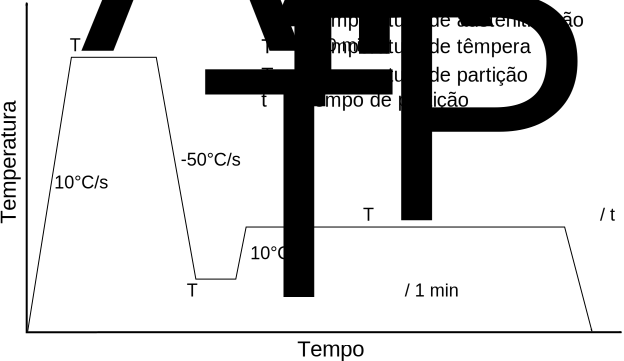
\includegraphics[height=8cm]{img/expproc_dil.pdf}
	\caption{Ilustração esquemática do ciclo térmico de Têmpera e Partição aplicado nas amostras de dilatometria.}
	\label{fig:expDil}
\end{figure}

O experimento para determinação da temperatura Ms consistiu do aquecimento da amostra até a temperatura de austenitização selecionada, seguindo rampa de aquecimento de 10 °C/s, sendo mantida nesta temperatura por 1800 segundos. Em seguida, a amostra foi resfriada até a temperatura de -100 °C sob taxa de resfriamento de --50 °C/s utilizando gás He refrigerado por $N_2$ líquido. O resfriamento até esta temperatura permitiu que a curva da transformação martensítica fosse determinada por completo. Para que o resfriamento até temperaturas abaixo de zero pudesse ser realizado no equipamento, a geometria da amostra utilizada foi de cilindro oco, como representado na figura \ref{fig:CPdil}b.

\subsection{Difra\c{c}\~{a}o de raios X \enfase{in situ}}

Tratamentos térmicos com acompanhamento em tempo real (\enfase{in situ}) da evolução de fases por difração de raios X gerados por fonte de luz síncrotron foram realizados na estação experimental \siglaestrangeira{XTMS}{X-ray Scattering and Thermo-Mechanical Simulation}, operada conjuntamente pelo \sigla{LNNano}{Laboratório Nacional de Nanotecnologia}  e pelo \sigla{LNLS}{Laboratório Nacional de Luz Síncrotron} na cidade de Campinas. A instalação da linha XTMS consiste de um avançado simulador termomecânico especialmente construído para ser usado em experimentos de difração de raios X. O simulador, chamado de Gleeble\textregistered{} 3S50, foi desenvolvido em cooperação da empresa estadunidense \siglaestrangeira{DSI}{Dynamic Systems Inc.} e de corpo técnico-científico do LNNano com o propósito de efetuar testes termomecânicos com controle de temperatura e solicitação mecânica em amostras macroscópicas, enquanto aquisições simultâneas de difração de raios X são obtidas. %A figura xx mostra a configuração da instalação no blablabla

No interior da câmara do simulador Gleeble os corpos de prova são presos por garras de cobre, por meio das quais é conduzida corrente elétrica para aquecimento das amostras por efeito Joule. O controle da potência é feito por algoritmo proporcional integral derivativo (PID), sendo que a resposta de temperatura é obtida por meio de termopares (tipo K, Alumel/Cromel) soldados às amostras.

A instalação conta com um goniômetro de alta resolução montado ao redor do simulador. O goniômetro é montado sobre uma mesa de alinhamento que permite o posicionamento do plano de difração sobre a superfície da amostra. Os detetores para contagem de fótons ficam localizados no goniômetro e podem ser posicionados em ângulos entre 0 e 150° e a uma distância mínima da superfície da amostra de 361 mm. Neste trabalho, foram utilizados dois detetores Mythen 1K, cada um possuindo 1280 canais de aquisição (pixels) de 50 $\mu$m de largura. Na distância mínima de trabalho, cada detetor cobre uma faixa de ângulos de aproximadamente 10°, totalizando um ângulo de cobertura de cerca de 20°.

Para os experimentos, corpos de prova do ferro fundido foram usinados na geometria esquematizada na figura \ref{fig:CPXTMS}. Durante o posicionamento das amostras no interior da câmara do simulador procurou-se estabelecer o ângulo $\omega$ de 15° entre a superfície da amostra e o feixe incidente de raios X. Em sequência, as amostras foram submetidas a ciclos de Têmpera e Partição segundo as condições de tratamento térmico pré-determinadas.

\simbolo{$\omega$}{Ângulo estabelecido entre o feixe de raios X incidente e a superfície da amostra}

Assim como nos ensaios de dilatometria realizados no dilatômetro Bähr, as amostras foram austenitizados durante 30 min, resfriadas até as temperaturas de têmpera e em seguida reaquecidas até as temperaturas de partição, em que foram mantidas durante 1800 segundos. Nas etapas de resfriamento não foi utilizado resfriamento forçado por meio convectivo, de modo que a extração de calor foi feita unicamente por meio das garras de cobre em contato com os corpos de prova. Consequentemente, taxas de resfriamento inferiores às obtidas no dilatômetro Bähr foram conseguidas no simulador Gleeble. Contudo, análise metalográfica posterior mostrou que a taxa de resfriamento utilizada foi suficiente para garantir a transformação martensítica na etapa de têmpera.

\begin{figure}
	\includegraphics[width=14cm]{img/CPXTMS.pdf}
	\caption{Desenho esquemático do corpo de prova utilizado na estação experimental XTMS. Dimensões em  milímetros.}
	\label{fig:CPXTMS}
\end{figure}

Paralelamente à realização dos tratamentos térmicos foram feitas aquisições de difração de raios X. A energia do feixe foi estabelecida em 12 keV, equivalente ao comprimento de onda $\lambda = 1,033\text{\AA}$, utilizando monocromador de Si(111). As fendas de limitação de fluxo de fótons foram ajustadas para permitirem que apenas uma região de 2 x 0,5 mm\textsuperscript{2} do feixe incidisse sobre a superfície da amostra. Durante as aquisições em tempo real, o goniômetro foi fixado no ângulo 2$\theta$ de 31° e os detetores Mythen foram aproximados até a distância mínima de trabalho de 361 mm. Nesta configuração, os detetores cobriram a faixa de ângulos de difração de 26 a 47°, na qual foi possível monitorar a evolução dos picos de difração (110) e (200) da ferrita e (111) e (200) da austenita em tempo real.

\simbolo{2$\theta$}{Ângulo de difração} %definir tth melhor aqui.

Dependendo da etapa do tratamento térmico, foram utilizados diferentes tempos e frequências de aquisição de dados. Durante a etapa isotérmica de partição, cuja análise é enfatizada neste trabalho, aquisições foram feitas usando tempo de exposição de 3 segundos, espaçadas a cada 0,5 segundos. Ao final da etapa de partição e do tratamento térmico foram feitas varreduras do ângulo de difração entre 26 e 86° a 10 segundos de exposição por passo, de modo a obter um número de picos de difração substantivo para quantificação das fases. A figura \ref{fig:esqXTMS} ilustra a programação do experimento na instalação XTMS.

\begin{figure}
	\includegraphics[height=10cm]{img/expproc_XTMS.pdf}
	\caption{Ilustração esquemática do teste programado na instalação XTMS.}
	\label{fig:esqXTMS}
\end{figure}

Antes de cada experimento a câmara do simulador Gleeble foi evacuada por um sistema de vácuo composto de bomba mecânica e difusora. Os níveis de vácuo atingidos foram consistentemente inferiores a $1 \times 10^{-2}$ torr. Um bom nível de vácuo é imprescindível para que a oxidação e a descarbonetação do material em sua superfície sejam evitadas durante o aquecimento e a aquisição dos difratogramas.

\subsubsection{An\'{a}lise dos resultados de DRX}

Uma vez que a amostra fica posicionada em um ângulo $\omega$ fixo em relação ao feixe de raios X, a geometria de difração $\omega$--$2\theta$ utilizada difere fundamentalmente das geometrias convencionais dos métodos de Bragg-Brentano ($\theta$--$2\theta$) e Debye-Scherrer (feixe transmitido). A interpretação dos padrões de difração, no entanto, seguiu procedimentos semelhantes de indexação e determinação dos parâmetros de rede das fases.

A análise dos difratogramas obtidos durante os tratamentos isotérmicos foi feita por meio de rotinas programadas em Rscript. Os picos de difração obtidos foram ajustados segundo a equação de distribuição Gaussiana (equação \ref{eq:Gaussiana}) que representa uma função sino que descreve o formato os picos de difração. O autor é ciente que para esta tarefa costuma ser utilizada uma função do tipo Pseudo-Voigt, que descreve melhor o alargamento instrumental associado aos picos de difração. Todavia, devido ao custo de processamento computacional e problemas no ajuste de picos superpostos utilizando essa função, optou-se pelo uso de perfis Gaussianos, que demonstraram fornecer resultados satisfatórios.

\begin{equation}
	I = I_0 \exp{\left[-\left(\frac{2\theta - 2\theta_0}{w}\right)^2\right]} + bck
	\label{eq:Gaussiana}
\end{equation}

Na equação \ref{eq:Gaussiana}, $I$ corresponde à intensidade de difração observada em função do ângulo $2\theta$, $I_0$ é a intensidade máxima medida no ângulo de difração $2\theta_0$, $w$ é a largura do pico Gaussiano e $bck$ contabiliza o sinal de fundo (\enfase{background}), que tem seu valor assumido como constante. As áreas integradas ($A_{hkl}$) sob os picos foram calculadas pela integração da curva Gaussiana usando a equação \ref{eq:intGauss}, sendo convertidas para frações volumétricas de fases pela equação \ref{eq:fracDRX}, conforme metologia descrita por \citaremsentenca{Cullity2001}.

\begin{align}
	A &= \int\limits_{-\infty}^{\infty} I_0 \exp{\left[-\left(\frac{2\theta - 2\theta_0}{w}\right)^2\right]} d \theta \nonumber \\
	&= I_0 |w| \sqrt{\pi}
	\label{eq:intGauss}
\end{align}

\begin{equation}
	f^\gamma = 1 - f^\alpha = \frac{\sum A_{hkl}^\gamma/R_{hkl}^\gamma}{\sum A_{hkl}^\alpha/R_{hkl}^\alpha + \sum A_{hkl}^\gamma/R_{hkl}^\gamma}
	\label{eq:fracDRX}
\end{equation}

A equação \ref{eq:fracDRX} faz uso dos coeficientes $R_{hkl}$ que contabilizam o efeito dos fatores que compõem o cálculo da intensidade teórica dos picos de difração. Na tabela \ref{tab:fatoresR} são apresentados os valores de $R_{hkl}$ utilizados para quantificação das fases neste trabalho.

\begin{table} %REVISAR ANTES DE IMPRIMIR!
	\caption{Coeficientes $R_{hkl}$ calculados para as fases ferrita ($\alpha$) e austenita ($\gamma$) do ferro puro\cite{Cullity2001}.}
	\begin{tabular}{c c c ' c c c}
	\thickhline
	Fase & hkl & $R_{hkl}$ & Fase & hkl & $R_{hkl}$\\
	\hline
	& 110 & 1840 & & 111 & 1351\\
	& 200 & 288,6 & & 200 & 644,3\\
	$\alpha$ & 211 & 530,0 & $\gamma$ & 220 & 376,7\\
	& 220 & 142,5 & & 311 & 390\\
	& 310 & 172,8 & & 222 & 107,9\\
	\thickhline
	\end{tabular}
	\label{tab:fatoresR}
\end{table}

A variação do parâmetro de rede da austenita ao longo do tratamento isotérmico também foi avaliada pelos resultados de DRX. A partir do cálculo do espaçamento interplanar $d_{hkl}$ pela lei de Bragg (equação \ref{eq:Bragg}), o parâmetro de rede da austenita $a^\gamma$ foi determinado pela equação \ref{eq:parametroRede}, que, para sistemas cristalinos cúbicos, estabelece a relação entre o parâmetro de rede da fase e a distância interplanar entre planos de índices de Miller $hkl$.

\begin{equation}
	n\lambda = 2d_{hkl}\,sen(\theta_0)
	\label{eq:Bragg}
\end{equation}

\begin{equation}
	d_{hkl}^\gamma = \frac{a^\gamma}{\sqrt{h^2 + k^2 + l^2}}
	\label{eq:parametroRede}
\end{equation}

A variação do parâmetro de rede foi interpretada pelo enriquecimento em carbono da austenita durante a etapa de partição do tratamento T\&P. Dessa forma, a variação do teor de carbono foi estimada por meio da equação empírica obtida por \citaremsentenca{Dyson1970}, que leva em conta a variação do parâmetro de rede da austenita em função de sua composição química:

\begin{equation}
	a^\gamma = 3,5780 + 3,30\cdot10^{-2} \%w_C^\gamma + 9,5\cdot10^{-4} \%w_{Mn}^\gamma + 1,5\cdot10^{-3} \%w_{Cu}^\gamma
	\label{eq:DysonHolmes}
\end{equation}
%
em que $\%w_i^\gamma$ é a porcentagem em massa do elemento $i$ (= C, Mn, Cu) dissolvido na austenita. A equação original também descreve a contribuição de outros elementos no parâmetro de rede da austenita. No entanto, suas representações na equação acima foram poupadas, devido a seus baixos teores na liga estudada. Dyson e Holmes argumentam que o silício, que aparece em quantidade substancial no ferro fundido, apresenta efeito desprezível na distorção do reticulado da austenita e, por esse motivo, sua contribuição não foi incorporada à equação.

Uma vez que as aquisições foram feitas a temperaturas elevadas, para que os valores de $a^\gamma$ obtidos pelos difratogramas pudessem ser interpretados na temperatura ambiente pelo método descrito acima, previamente à aplicação da equação \ref{eq:DysonHolmes}, o efeito da expansão térmica no parâmetro de rede da austenita foi corrigido utilizando a equação desenvolvida por \citaremsentenca{VanBohemen2013b}:

\begin{equation}
	\frac{\Delta L^\gamma}{L_0^\gamma} = B_\gamma T + B_\gamma \Theta_D^\gamma \left[ \exp{\left( -\frac{T}{\Theta_D^\gamma} \right)}\right]
	\label{eq:expTermica}
\end{equation}

A equação \ref{eq:expTermica} descreve a variação de comprimento $\Delta L^\gamma$ de uma amostra completamente austenítica na temperatura absoluta $T$ em relação a seu comprimento $L_0^\gamma$ extrapolado para o estado de referência a 0 K. $B^\gamma$ e $\Theta_D^\gamma$ são constantes de ajuste determinadas pela regressão linear de dados disponíveis na literatura e valem $B^\gamma = 24,8 \times 10^{-6} K^{-1}$ e $\Theta_D^\gamma = 280 K$.

\subsection{Caracteriza\c{c}\~{a}o microestrutural}

Para análise da microestrutura das amostras, estas foram submetidas a preparação metalográfica, que consistiu do embutimento das amostras em baquelite, lixamento em lixa d'água até granulometria 1200 e subsequente polimento em pastas de diamante de 6, 3 e 1 $\mu$m. Por fim, as amostras foram submetidas a ataques metalográficos com reagentes químicos adequados para cada propósito. Para observação no microscópio óptico, as amostras foram pré-atacadas com o reagente Nital 2\% ($etanol + 2\%vol\,HNO_3$), sendo logo em seguida lavadas sob água corrente com detergente neutro e algodão, e subsequentemente imersas em solução do reagente Beraha ($3g\,K_2S_2O_5 + 10g\,Na_2S_2O_3 + 100mL\,H_2O$) por 60 segundos. O reagente Beraha, assim como outros reagentes que produzem ataques seletivos em ligas ferrosas, colore a ferrita, deixando-a marrom quando observada no microscópio óptico. De forma semelhante acontece com a martensita, que se apresenta tingida sob ação deste reagente. Por sua vez, a austenita fica isenta do ataque e, consequentemente, aparece branca nas micrografias\cite{MetalsVol9}. Para observação no \sigla{MEV}{Microscópio Eletrônico de Varredura}, as amostras foram apenas atacadas utilizando o reagente Nital 2\%.

Para obtenção de imagens de microscopia óptica foi utilizado um microscópio óptico Olympus BX60M com câmera CCD acoplada, localizado nas dependências do \sigla{LCMHC}{Laboratório de Caracterização Microestrutural Hubertus Colpaert} do \sigla{PMT-USP}{Departamento de Engenharia Metalúrgica e de Materiais da EPUSP}. As imagens de microscopia eletrônica de varredura foram obtidas tanto no microscópio de feixe de emissão de campo (MEV-FEG) FEI Inspect F50 com sistemas de \sigla{EDS}{Análise de Energia Dispersiva} e \sigla{EBSD}{Difração de Elétrons Retroespalhados} acoplados a ele. Estes equipamentos estão situados no \sigla{LabMicro}{Laboratório de Microscropia Eletrônica e de Força Atômica}, também vinculado ao PMT-USP.

\novasigla{MEV-FEG}{Microscópio Eletrônico de Varredura de Feixe de Emissão de Campo}